\documentclass[11pt]{beamer}
\usetheme{Berkeley}

\usepackage[utf8]{inputenc}
\usepackage[T1]{fontenc}
\usepackage{amsmath}
\usepackage{amsfonts}
\usepackage{amssymb}
\usepackage{graphicx}
\usepackage{xeCJK}


\author{何静}

\title{生产与运作管理实务}

\logo{
\includegraphics[width=0.1\textwidth]{../share/logo}}

\institute{东莞职业技术学院}

\date{2016年2月23日}

\setbeamercovered{transparent}

\setlength{\parindent}{2em}
\setlength{\parskip}{1em}
\setlength{\baselineskip}{20pt}
\renewcommand{\baselinestretch}{1.25}

\begin{document}
	\maketitle
	
	\begin{frame}{目录}
		\tableofcontents
	\end{frame}
	
	\section{绪论}
	\begin{frame}{为什么要学习《生产与运作管理》}
		《生产与运作管理》是工商管理的专业核心课程。目的是使学生对生产运营管理的内容有全面的了解,掌握基本运作管理技术和方法,为将来进行生产或者服务管理打下良好的基础。
		
		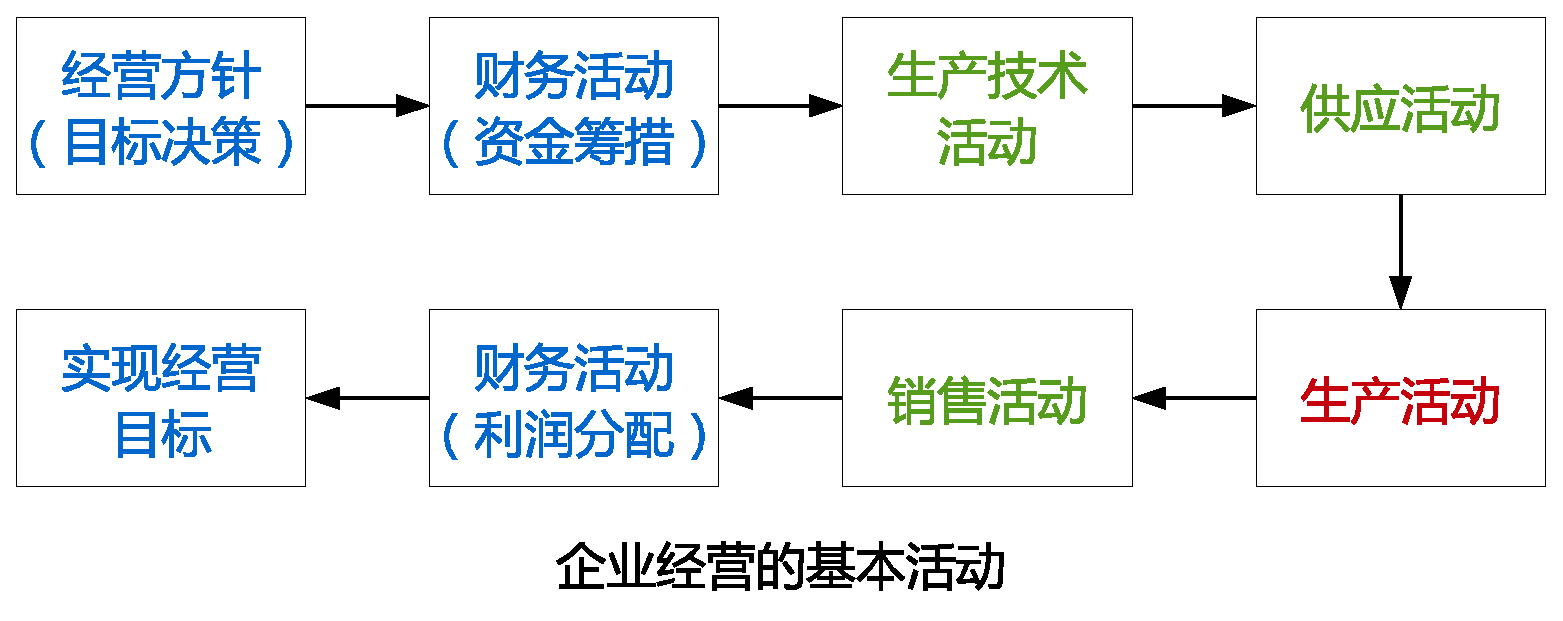
\includegraphics[width=0.9\textwidth]{img/生产活动}
	\end{frame}
	
	\begin{frame}{“生产与运作管理”在企业中的地位}
		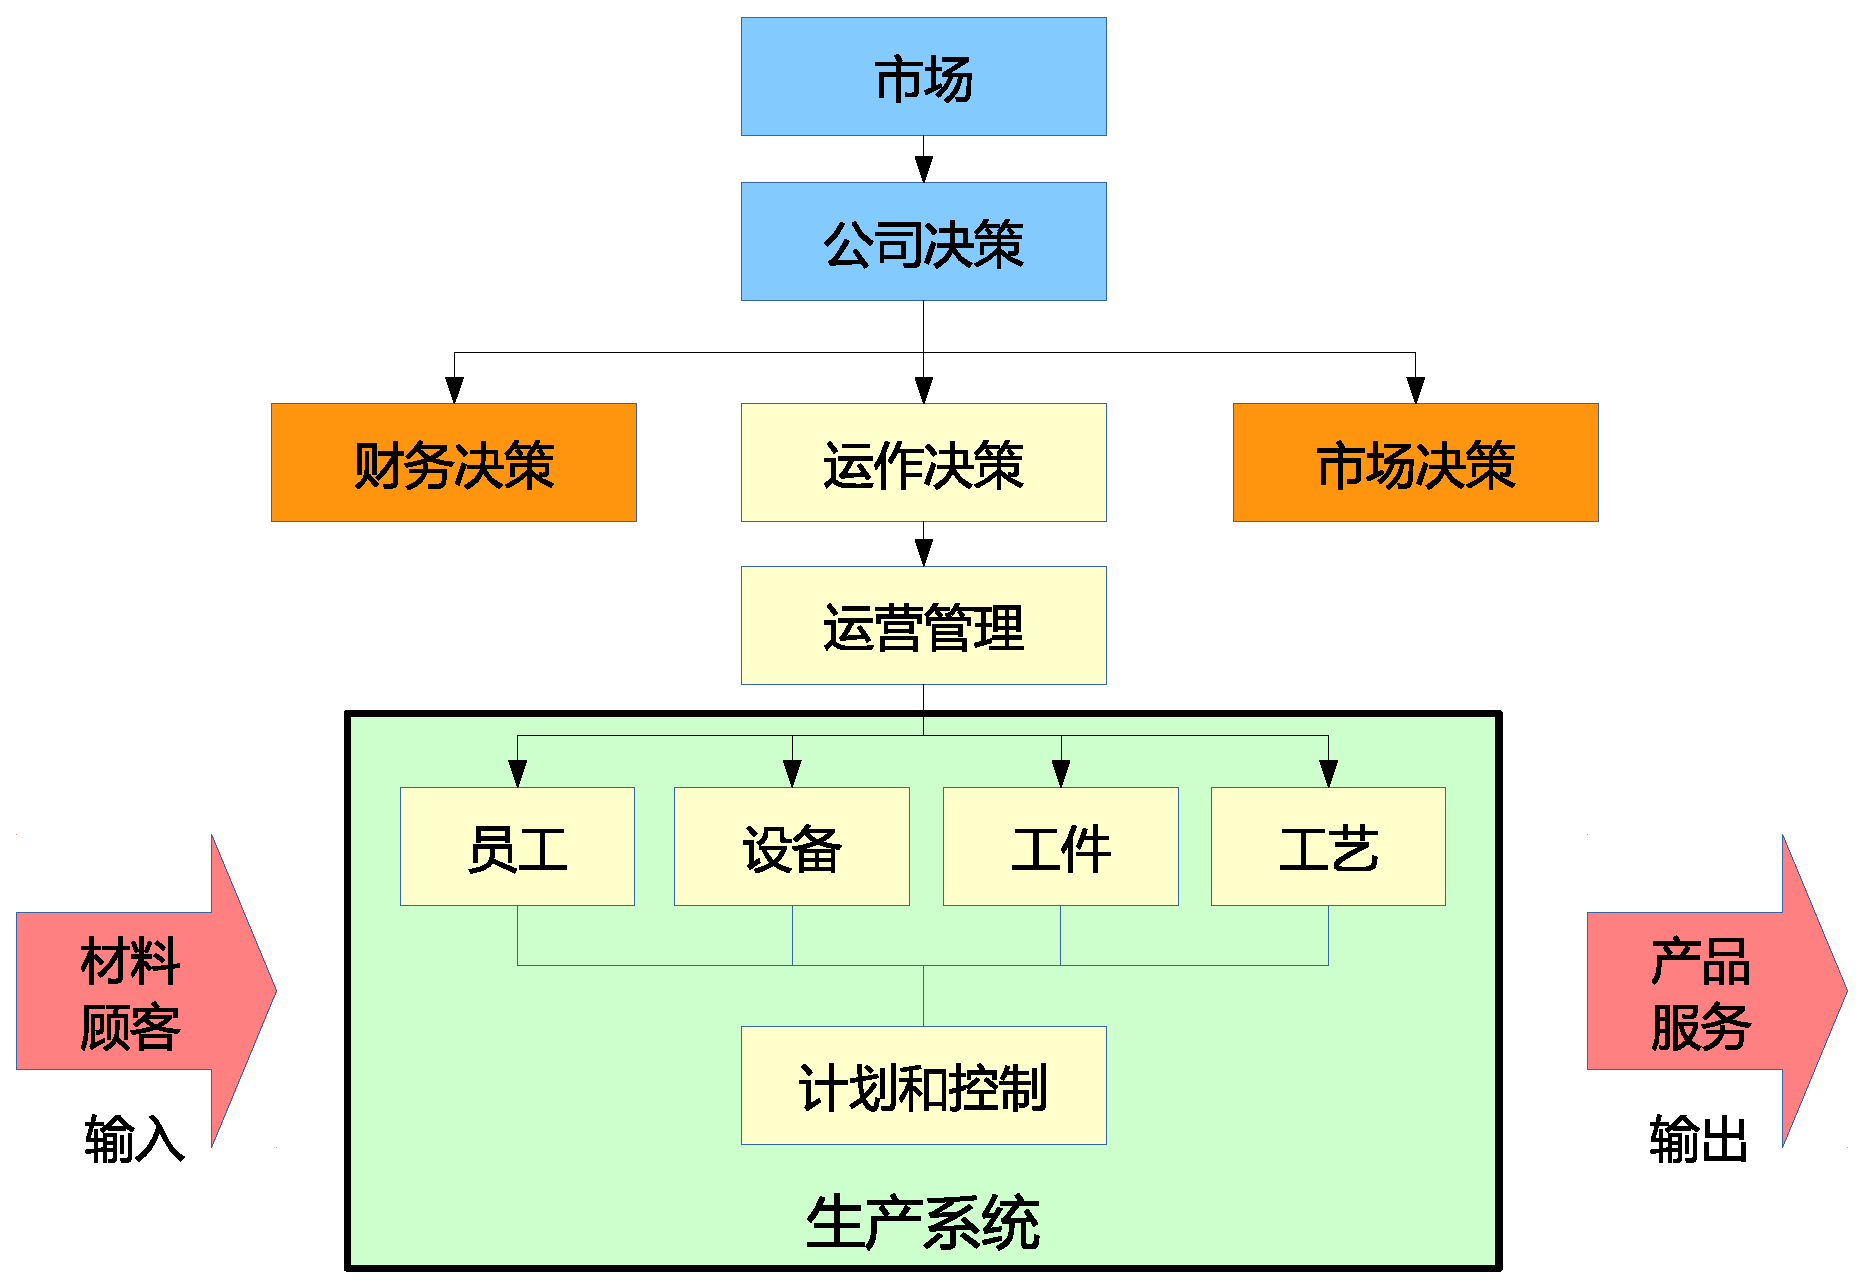
\includegraphics[width=0.9\textwidth]{img/生产系统}
	\end{frame}
	
	

\end{document}